\subsection{Backend Design}

I det følgende afsnit beskrives design overvejelser i forbindelse med udviklingen af systemets backend Web Api. Afsnittet vil give et overblik over hvilke resources/routes Web api’et stiller til rådighed. Efterfølgende forklares hvordan Data transfer objects vil blive anvendt, hvordan Authentication og Autherization vil blive håndteret, samt hvordan passwords vil blive hashed. Hertil vil en BackEndController klasse, som skal bruges på client siden blive redegjort for. Tilslut præsenteres applikationsmodeller over controller klasserne for de relevante User Stories, som består af en række sekvens og klasse diagrammer.\\

\subsubsection{Analyse konklusion}
I dette projekt vil give bedst mening at anvende mulighed 1 (REF TIL ANALYSE) med en backend bestående af ASP.NET og EF Core. Her fåes nemlig muligheden for at separere data resourcerne fra resten af applikationen samtidig med vi for en mere sikker og pålidelig håndtering af brugere samtidig med EF Core stadig understøttes til kommunikation med databasen i gennem LINQ.\\

\subsubsection{Routes}
Applikationens nødvendige routes kan inddeles i to under grupper ”Save”, som indeholder routes relateret til game state og ”User”, som indeholder routes relateret til brugeren. Alle routes som omhandler game state skal authorizes, mens routes, som omhandler brugeren tilader anonyme forespørgelser. Nedenfor er givet en oversigt over de forskellige routes med en tilhørende beskrivelse.\\

\textbf{Save:}\\
\begin{itemize}
\item GET: /api/Save
Denne route henter et sepcifikt gemt game state fra databasen, for den bruger som er logget ind.
\item POST: /api/Save\\
Denne route sender et scecifikt game state til databasen, for den bruger som er logget ind.
\item GET: /api/Save/Get List Of Saves\\
Denne route henter en liste af game states, for den bruger som er logget ind. 
\item GET: /api/Save/Get Room Description\\
Denne route henter en beskrivelse af det valgt rum i spillet.
\end{itemize}

\textbf{User:}\\
\begin{itemize}
\item POST: /api/User/Register\\
Denne route registrerer en ny bruger ved at gemme oplysninger om denne i databasen, og returnerer en JWT token. Når en bruger bliver registreret får den tildelt 5 pladser i databasen til game states.
\item POST: /api/User/Login\\
Denne route logger en bruger ind ved at tjekke bruger oplysninger med dem, som er registreret i databasen, denne route returnerer også en JWT token.
\end{itemize}

\subsubsection{Data Transfer Object:}

De data objekter som gemmes i SQL databasen vil indeholde nogle navigational properties, som bruges til at query data’en og til at opretter relationer mellem objekterne. Da disse properties ikke har nogen relevans for clienten oprettes der følgende DTO’er for modellerne User og Save som ses på \autoref{fig:Design-Backend-DTO}\\

\begin{figure}[H]
\centering
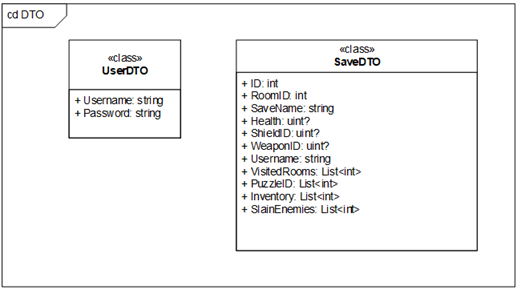
\includegraphics[width = \textwidth]{02-Body/Images/Backend_DTO.PNG}
\caption{klasse diagram over DTO'er for User og Save}
\label{fig:Design-Backend-DTO}
\end{figure}

På den måde kan man sikre at kun den nødvendige data sendes til clienten.\\

\subsubsection{Authentication/Authorization med JWT Token}
JWT (Jason Web Token) er et JSON object, som bruges til at validere (Authenticate), og til at afgøre hvorvidt en client har adgang til den givne data (Authorizing). En token består af tre dele en header, en payload og en signature.\\

\textbf{Header:}\\
Headeren består af en type og en hashing algoritme, typen vil for dette system være ”JWT” og algortimen vil være ”HmacSha256”.\\

\textbf{Payload:}\\

Payloaden indeholder såkaldte claims, der findes tre typer af claims reserved, public og private. Reserved er en række prædefineret claims som kan bruges til eksempelvis at sætte en tidsbegrænsning på den gældende. Public og private claims kan indeholde noget information omkring brugeren. I dette system benyttes private claims til at indeholde brugerens username, som så kan bruges til at genkende hvem den aktuelle token tilhører ved en forespørgsel.\\

\textbf{Signature:}\\
Signature bruges til at verificere hvem som er afsender af JWT’en, og til sikre at den ikke er blevet ændret undervejs. Her samles header, payload og en ”secret” som er en hemmelig string af tegn, kun Web Api'et kender.
For at generere denne token implementeres en funktion, som opretter en token efter de forhold som er beskrevet ovenfor.\\


\subsubsection{Hashing}
Under design fasen blev det besluttet at anvende hashing til at gemme en brugers password i databasen, for at øge sikkerheden. Sikkerhed var ellers ikke prioteret i vores MoSCoW analyse, for denne udgave af spillet.
Hashing af passwords går ud på at kryptere det gemte password i databasen. Det skal krypteres således at det ikke er muligt at dekryptere, samtidig med at det stadig kan valideres om det er et korrekt password, der modtages af en client. Når et password hashes anvendes et såkaldt ”salt”, som er en tilfældigt genereret string kobineret med password’et.\\

Til at Hashe passwords med anvendes Bcrypt (MANGLER REF), dette library stiller hashing af passwords til rådighed. Der findes en C\# udgave kaldet Bcrypt.Net  som vil blive anvendt. Helt præcist er det funktionen HashPassword(”password”, BcryptWorkfactor), denne funktion skal have en BcryptWorkfactor, hvilket er et tal der siger noget om hvor mange iterationer Bcrypt vil bruge på at generere det ”salt” til at hashe password’et med. Her anbefales det at bruge en værdi på 11, da det generelt set anses som tilstrækeligt niveau hvad angår sikkerhed.
Funktionen verify(”password”, hashedpassword) bruges til at verificere om et givent password svare til dets krypterede udgave.\\

\subsubsection{BackEndController på client siden}
Til brug af clienten for at tilgå backenden, skal der bruges en BackendController klasse, dennes ansvar vil være at udføre HTTP request/responses, og vil indeholde en funktion for hvert endpoint.\\
 
Klassen vil gøre brug af en HttpClient som er en klasse .Net stiller til rådighed til at håndtere HTTP request/responses. Da backenden kræver en JWT for at få adgang til endpoints, hvad angår loading og saving af game state, skal clienten også gemme JWT for den bruger som er logget ind, således at den kan blive sendt med de forskellige requests.


\subsection{Applikationsmodeller}
I dette afsnit gennemgåes applikationsmodeller for de enkelte user stories, der udarbejdes sekvensdiagrammer for at beskrive funktionalitet og klasse diagrammer til at beskrive indeholdet og sammen spillet imellem klasserne. Applikationsmodellerne deles op efter controllere, en for UserControlleren og en for SaveControlleren. Fokuset vil her ligge på controller klasserne, for en beskrivelse af DAL komponenterne henvises til database design afsnitet (MANGLER REF TIL DAL).\\

\subsubsection{Applikationsmodel User Controller}
\textbf{User Story 1: Log in}\\
Når clienten udfører en HTTP request med URL’en : ” https://localhost:7046/api/User/Login”, udføres følgende aktioner som fremgår af sekvensdiagrammet på \autoref{fig:Design-Backend-Sekvens-1}\\ 

\begin{figure}[H]
\centering
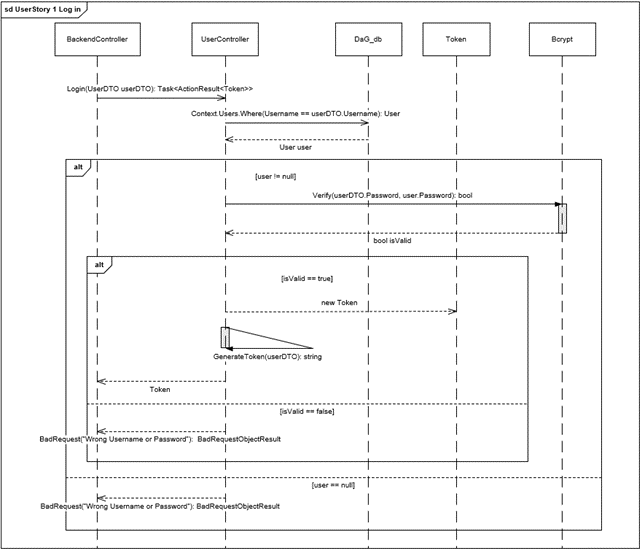
\includegraphics[width = \textwidth]{02-Body/Images/Backend_sekvens_1.PNG}
\caption{Sekvensdiagram som viser funktionaliteten i User Story 1 Log in}
\label{fig:Design-Backend-Sekvens-1}
\end{figure}

Authentication controlleren fra C3 modellen hedder her “UserController” og har til opgave at gøre det muligt for en bruger at registrere sig og logge ind. Login implementeres i Login() funktionen, som er det endpoint clienten kalder for at logge ind. Her bliver der tjekket om det indtastede brugernavn findes i databasen. Hvis brugernavnet findes, så bliver adgangskoden tjekket med funktionen verify fra Bcrypt klassen, og passer den, bliver der returneret en JWT token. Hvis brugernavnet derimod allerede eksiterer eller adgangskoden ikke er korrekt retuneres en fejlmeddelse.\\

\textbf{User Story 2: Opret Bruger}\\
Når clienten udfører en HTTP request med URL’en : ” https://localhost:7046/api/User/Register”, udføres følgende aktioner som fremgår af sekvensdiagrammet på \autoref{fig:Design-Backend-Sekvens-2}\\

\begin{figure}[H]
\centering
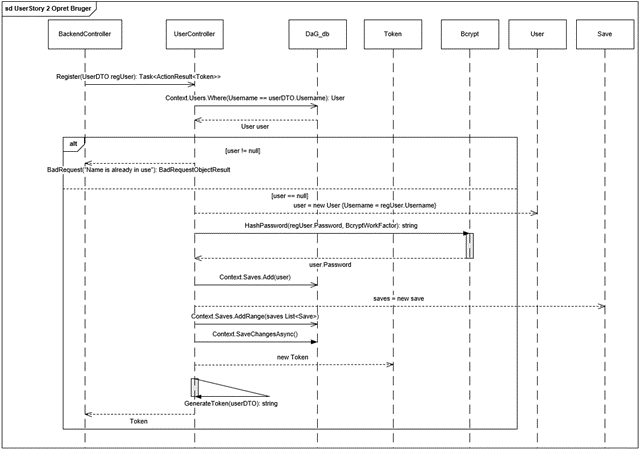
\includegraphics[width = \textwidth]{02-Body/Images/Backend_sekvens_2.PNG}
\caption{Sekvensdiagram som viser funktionaliteten i User Story 2 Opret Bruger}
\label{fig:Design-Backend-Sekvens-2}
\end{figure}

For at kunne logge ind skal det være muligt at oprette en bruger til dette laves en Register(UserDTO regUser) funktion. Denne starter med at checke om brugernavnet er optaget. Er den det, returneres der en fejlmeddelelse, og ellers registreres brugeren. Dernæst bliver det valgte kodeord ”hashed”, således at der opnås en vis sikkerhed i systemet. Når der oprettes en ny bruger skal denne have tildelt 5 pladser i databasen til sine gemte spil, dette sker ved at der oprettes en liste af saves der indeholder 5 nye saves, disse gemmes med contexten i SQL databasen. Hvis alt går godt retuneres en JWT token.\\

\textbf{Samlet Klasse diagram over User Story 1 og 2}\\

På \autoref{fig:Design-Backend-Klasse-1-2} kan ses en oversigt over de klasser, metoder og attributter, som anvendes i udførelsen af User story 1 og 2. Hertil anvendes også klassen Bcrypt som ikke er taget med, da den blot er brugt udefra, detaljer om Bcrypt kan ses i afsnitet ovenover(MANGLER REF).\\

\begin{figure}[H]
\centering
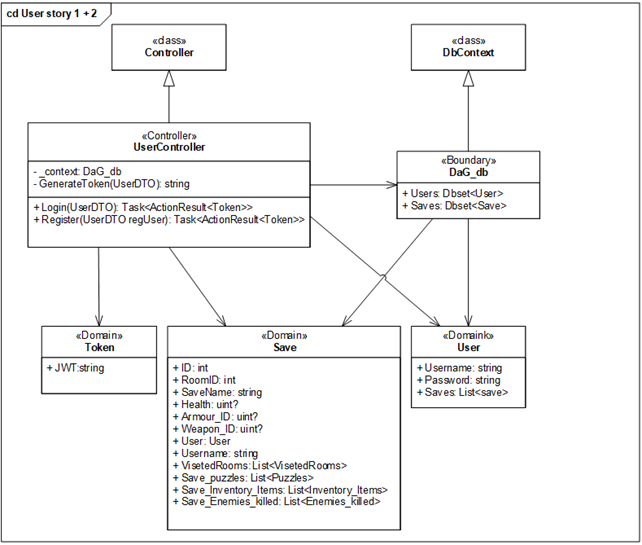
\includegraphics[width = \textwidth]{02-Body/Images/Backend_klasse_1_2.PNG}
\caption{Samlet klasse diagram over User story 1 og 2}
\label{fig:Design-Backend-Klasse-1-2}
\end{figure}

\subsubsection{Applikationsmodel Save Controller}
\textbf{User Story 7: Exit Menu -\g Save and Exit}\\
Load/save controlleren fra C3 modellen er blevet til en enkelt controller, som kaldes for ”SaveController”. Denne controller har til ansvar at gemme et spil, men samtidig også være i stand til at kunne hente gemte spil, altså at loade dem.
Når clienten udfører en HTTP request med URL’en : ” https://localhost:7046/api/Save”, udføres følgende aktioner som fremgår af sekvensdiagrammet på \autoref{fig:Design-Backend-Sekvens-7}\\

\begin{figure}[H]
\centering
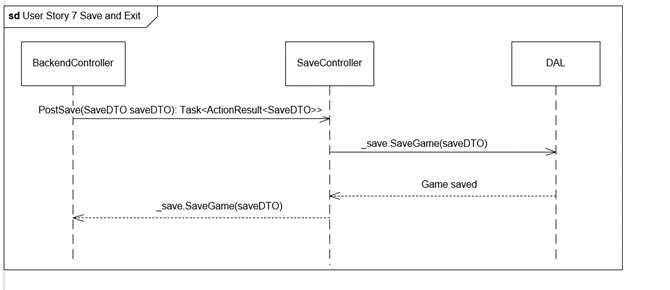
\includegraphics[width = \textwidth]{02-Body/Images/Backend_sekvens_7.PNG}
\caption{sekvensdiagram over User Story 7 Save and Exit}
\label{fig:Design-Backend-Sekvens-7}
\end{figure}

Der bruges en httpPost funktion kaldet PostSave som gemmer et nyt spil i databasen ved at ligge det modtagene gamestate fra parameter listen ind i et funktionskald SaveGame() i DAL klassen, som så sørger for at gemme spillet i databasen på den korrekte måde.\\

\textbf{User Story 17: Exit Menu -\g Save and Exit}\\

Når clienten udfører en HTTP request med URL’en : ” https://localhost:7046/api/Save/Get List Of Saves”, udføres følgende aktioner som fremgår af sekvensdiagrammet på \autoref{fig:Design-Backend-Sekvens-17}\\

\begin{figure}[H]
\centering
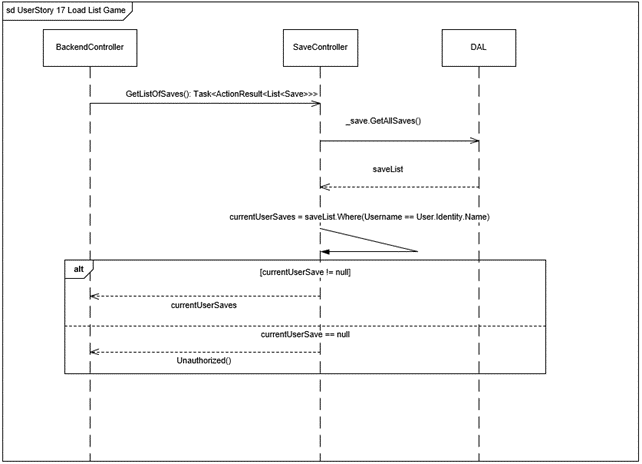
\includegraphics[width = \textwidth]{02-Body/Images/Backend_sekvens_17.PNG}
\caption{Sekvensdiagram over User Story 17 Main Menu -\g Load List Game}
\label{fig:Design-Backend-Sekvens-17}
\end{figure}

Da vi gerne vil gøre det muligt at have 5 save games pr. profil, skal det naturligvis være muligt at kunne vælge mellem de forskellige saves, til dette laves funktion GetListOfSaves(). Clienten kalder her GetListOfSaves() som er et HttpGet endpoint, denne funktion henter alle saves i DAL klassen ved at kalde GetAllSaves(). SaveController finder så de gemte spil i listen hvor brugernavnet passer med den burger, som er logget ind ved brug af User.Identity som stilles til rådighed af ControllerBase klassen, her i kan claims for den nuværende JWT nemlig findes.\\

\textbf{UserStory 18 : Main Menu -\g Load Game -\g Load}\\
Når clienten udfører en HTTP request med URL’en :” https://localhost:7046/api/Save?id={id}”, udføres følgende aktioner som fremgår af sekvensdiagrammet på \autoref{fig:Design-Backend-Sekvens-18}\\

\begin{figure}[H]
\centering
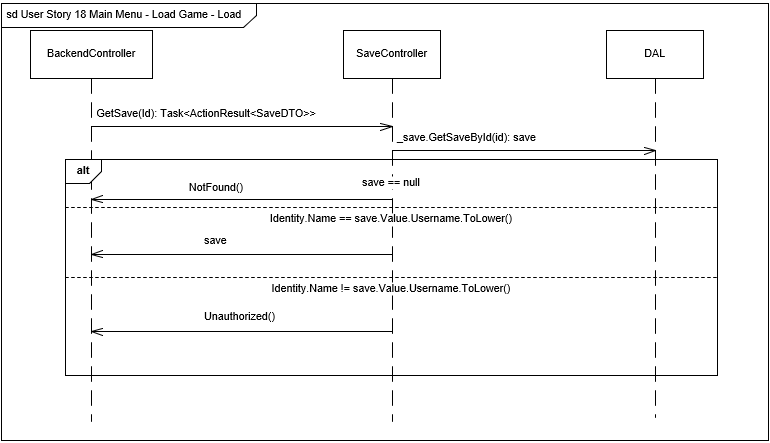
\includegraphics[width = \textwidth]{02-Body/Images/Backend_sekvens_18.PNG}
\caption{Sekvens diagram over User story 18 Main Menu -> Load Game -> Load}
\label{fig:Design-Backend-Sekvens-18}
\end{figure}

\textbf{User Story 19 : Main Menu -\g Load Game -\g Delete Game}\\

Under design fasen blev det besluttet at overskrive gemte saves fremfor at slette og lave et nyt, da et saves Id på den måde ikke ændret sig i databasen når man lavede et nyt save. Derfor er User story 19 som omhandler Delete game ikke taget med i design fasen.\\

\textbf{Samlet klasse diagram over User story 7, 17 og 18}\\
Et Samlet klasse diagram for User story 7, 17 og 18 kan ses på \autoref{fig:Design-Backend-Sekvens-7-17-18}\\

\begin{figure}[H]
\centering
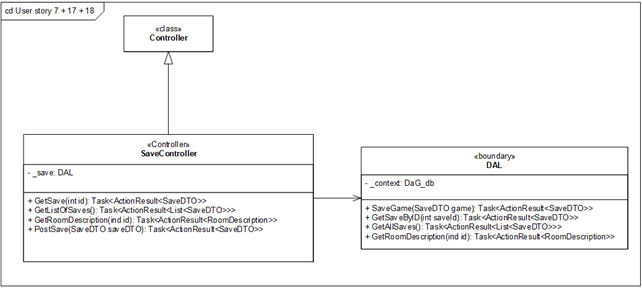
\includegraphics[width = \textwidth]{02-Body/Images/Backend_klasse_7_17_18.PNG}
\caption{Samlet klasse diagram for User story 7, 17 og 18}
\label{fig:Design-Backend-Sekvens-7-17-18}
\end{figure}

Udover de funktioner som bliver brugt i User stories, tilføjes der er en funktion GetRoomDescription, som blot henter en beskrivelse af det rum brugeren befinder sig i.\\


\subsubsection{Konklusion}

Backenden er blevet designet såldedes at den kan håndtere alle de nødvendige kald for at opfylde user stories omkring brugere og gemte spil, dette er beskrevet igennem appilationsmodeller. JWT tokens anvendes til Authentication og Authorization. Til hashing af passwords anvendes Bcrypt. Hertil er BackendControlleren klassen blevet introduceret på clienten, som står for HTTP request/response.\\ 


\newpage
